\documentclass[letterpaper]{article}

\usepackage[english]{babel}
\usepackage[utf8]{inputenc}
\usepackage{amsmath}
\usepackage{graphicx}
\usepackage[colorinlistoftodos]{todonotes}
\def\MLine#1{\par\hspace*{-\leftmargin}\parbox{\textwidth}{\[#1\]}}

\title{Crime and Punishment | final project for CAPP 30255}

\author{Carlos Grandet and Hector Salvador}

\date{\today}

\begin{document}
\maketitle

\begin{abstract}
We made a first version of a question-answering program that retrieves a set of potential answers to questions like: What is the penalty for committing murder?. We use the 300 current Mexican federal laws, specifically attempting to retrieve criminal and administrative sentences (e.g. jail years, fines, political disablement). We implement this machine in Python, using the framework described by Jurafsky and Martin \cite{jurafsky}. We show our results, challenges, and potential next steps to improve our machine.
\linebreak

\textbf{Keywords:} question-answering machine, natural language processing, Mexican federal laws, text analysis.
\end{abstract}

\section{Introduction}
\label{sec:introduction}

We thought a question answering machine was a good idea for a final project because:
\begin{itemize}
\item This could empower people to look if certain sentences or penalties are real. In a corrupt country like Mexico, sometimes people don't know if the punishment they're receiving is even legally sound. A lot of people would not dare to contradict a judge or a lawyer, just because they don't have any education to understand laws. 
\item It's hard to read lots of laws at once. Hector worked in the past with regulations in energy and had to quickly understand 14 new laws when they came out. This took him a very long time to read, especially since laws sometimes use a particular language and understanding them correctly takes a lot of time.
\item Since we're Mexican, we wanted to do a text analysis project in Spanish. We were very happy to  be able to apply many of the concepts we learned in class: dynamic programming, word2vec, n-gram models with Hidden Markov Models, and information retrieval (IR).
\end{itemize}


\section{Framework}
\label{sec:theory}

\subsection{Overview}

We followed the three stages of an IR-based factoid question answering machine (figure \ref{fig:pipeline}). We scraped 300 Mexican federal laws from the Mexican congress website: http://www.diputados.gob.mx/LeyesBiblio/index.htm. We then used these documents to create passages (a smaller unit of documents) that would be retrieved by an IR algorithm. Finally, we prioritize these passages, using a combination of BM25 and the probability of the passage containing an answer. Because of time constraints (we had less than 1/3 of a 10-week quarter to work on this project), we could not do any work on the answer processing part of the pipeline.

\begin{figure}
\centering
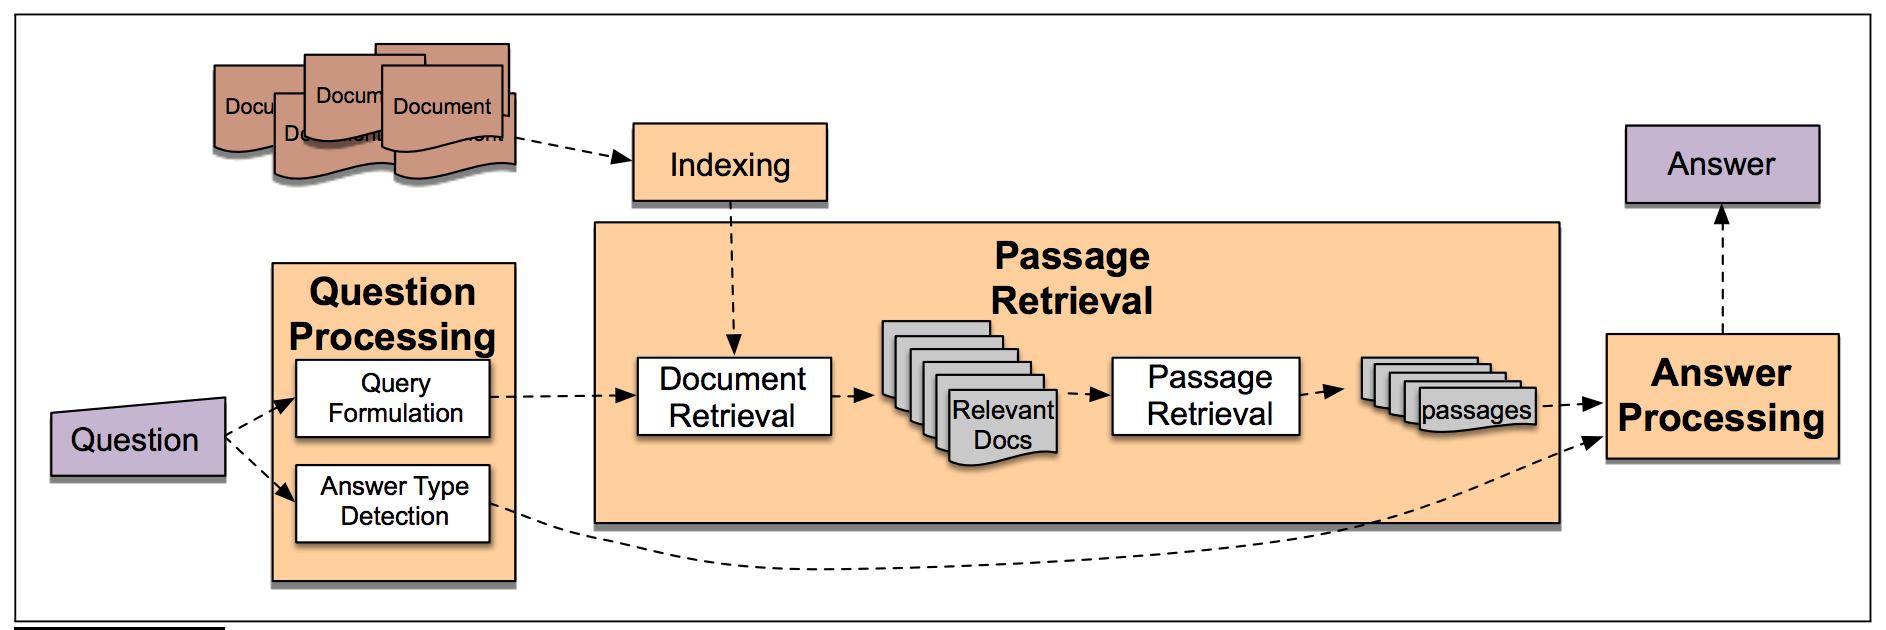
\includegraphics[width=1\textwidth]{pipeline.png}
\caption{\label{fig:pipeline}IR-based factoid question answering has three stages: question processing, passage retrieval, and answer processing. This is Figure 28.2 from \cite{jurafsky}, Chapter 28.1.1.}
\end{figure}

\subsection{Document creation}
Scraping was done using \texttt{scrape.py}. Laws were available both in \texttt{pdf} and \texttt{doc} files. Two methods were tested to convert the files to \texttt{txt} files that could be processed in Python. 

First we tried converting \texttt{pdf} files to \texttt{txt} using out-of-the-box packages (e.g. using \texttt{pdftotext} utility in the command line). Unfortunately, Mexican laws have a ton of useless text as headers and footnotes \ref{fig:header}, which are repeated over all documents. This introduced a lot of noise in our models, so we tried next using \texttt{doc} files.

We attempted unsuccessfully to just open \texttt{doc} files in Python. There were a lot of binary characters that made reading and text processing difficult. Maybe it was our lack of experience opening files, but we could not find a way to retrieve only the text we needed, especially since many characters have accents in Spanish. We also tried using \texttt{antiword} and \texttt{python-docx}, but we kept having installation errors, even using a virtual environment\footnote{Using a macOS Sierra 10.12.3 and python 3.5}.

After spending several hours, we opted to manually convert \texttt{doc} files to \texttt{txt} manually. These can all be found in the folder called \texttt{/leyes/*}.

\begin{figure}
\centering

\includegraphics[width=1\textwidth]{header.png}
\caption{\label{fig:header}Example of the top part of a Mexican Law saved as a doc file. Notice the headers, the titles, subtitles, and additional text that is non-informative.}
\end{figure}

\subsection{Question processing}
Explain the IQHE in your own words. What does the density of states look like in a 2-DEG when $B=0$? What are Landau levels and how do they arise? What are edge states? What does the electron transport look like when you change the magnetic field? What do you expect to measure?

\subsection{Document retrieval}


\subsection{What didn't work?}

\section{Results}
\subsection{Why}
Explain a step-by-step recipe for fabrication here. How long did you etch and why? What is an Ohmic contact?
\subsection{Experimental set-up}
Explain the experimental set-up here. Use a schematic picture (make it yourself in photoshop, paint, ...) to show how the components are connected. Briefly explain how a lock-in amplifier works.

\section{Future Work}
Show a graph of the longitudinal resistivity ($\rho_{xx}$) and Hall resistivity ($\rho_{xy}$) versus magnetic field, extracted from the raw data shown in figure \ref{fig:data}. You will have the link to the data in your absalon messages, if not e-mail Guen (guen@nbi.dk). Explain how you calculated these values, and refer to the theory.

\begin{figure}
\centering
\includegraphics[width=1\textwidth]{raw_data.png}
\caption{\label{fig:data}Raw (unprocessed) data. Replace this figure with the one you've made, that shows the resistivity.}
\end{figure}

\subsection{Classical regime}
Calculate the sheet electron density $n_{s}$ and electron mobility $\mu$ from the data in the low-field regime, and refer to the theory in section \ref{sec:theory}. Explain how you retrieved the values from the data (did you use a linear fit?).
Round values off to 1 or 2 significant digits: 8.1643 ~= 8.2. Also, 5e-6 is easier to read than 0.000005.

!OBS: This part is optional (only if you have time left).
Calculate the uncertainty as follows: \newline $u(f(x, y, z)) = \sqrt{(\frac{\delta f}{\delta{x}} u(x))^{2} + (\frac{\delta f}{\delta{y}} u(y))^{2} + (\frac{\delta f}{\delta{z}} u(z))^{2}}$, where $f$ is the calculated value ($n_{s}$ or $\mu$), $x, y, z$ are the variables taken from the measurement and $u(x)$ is the uncertainty in x (and so on).

\subsection{Quantum regime}
Calculate $n_{s}$ for the high-field regime.
Show a graph of the longitudinal conductivity ($\rho_{xx}$) and Hall conductivity($\rho_{xy}$) \textbf{in units of the resistance quantum} ($\frac{h}{e^{2}}$), depicting the integer filling factors for each plateau.
Show a graph of the plateau number versus its corresponding value of $1/B$. From this you can determine the slope, which you use to calculate the electron density.
Again, calculate the uncertainty for your obtained values.

\section{Discussion 1/2-1 page}
Discuss your results. Compare the two values of $n_{s}$ that you've found in the previous section. Compare your results with literature and comment on the difference. If you didn't know the value of the resistance quantum, would you be able to deduce it from your measurements? If yes/no, why?

\newpage
\section{Some LaTeX tips}
\label{sec:latex}
\subsection{How to Include Figures}

First you have to upload the image file (JPEG, PNG or PDF) from your computer to writeLaTeX using the upload link the project menu. Then use the includegraphics command to include it in your document. Use the figure environment and the caption command to add a number and a caption to your figure. See the code for Figure \ref{fig:frog} in this section for an example.

\begin{figure}
\centering
\includegraphics[width=0.3\textwidth]{frog.jpg}
\caption{\label{fig:frog}This frog was uploaded to writeLaTeX via the project menu.}
\end{figure}

\subsection{How to Make Tables}

Use the table and tabular commands for basic tables --- see Table~\ref{tab:widgets}, for example.

\begin{table}
\centering
\begin{tabular}{l|r}
Item & Quantity \\\hline
Widgets & 42 \\
Gadgets & 13
\end{tabular}
\caption{\label{tab:widgets}An example table.}
\end{table}

\subsection{How to Write Mathematics}

\LaTeX{} is great at typesetting mathematics. Let $X_1, X_2, \ldots, X_n$ be a sequence of independent and identically distributed random variables with $\text{E}[X_i] = \mu$ and $\text{Var}[X_i] = \sigma^2 < \infty$, and let

\begin{equation}
S_n = \frac{X_1 + X_2 + \cdots + X_n}{n}
      = \frac{1}{n}\sum_{i}^{n} X_i
\label{eq:sn}
\end{equation}

denote their mean. Then as $n$ approaches infinity, the random variables $\sqrt{n}(S_n - \mu)$ converge in distribution to a normal $\mathcal{N}(0, \sigma^2)$.

The equation \ref{eq:sn} is very nice.

\subsection{How to Make Sections and Subsections}

Use section and subsection commands to organize your document. \LaTeX{} handles all the formatting and numbering automatically. Use ref and label commands for cross-references.

\subsection{How to run the code}

Before running the code, make sure that the \texttt{txt} files are in folder called leyes and that the file called \texttt{docnames.csv} is in the folder called \texttt{doc}.

\begin{enumerate}
\item Open a Python shell, preferably ipython.
\item If you want to download the \texttt{doc} files, run \\ \texttt{\$ run scrape.py} \\ then call \\ \texttt{\$ go()} \\ This will download the \texttt{doc} files in the folder called \texttt{/doc}.
\end{enumerate}

\begin{description}
\item[Word] Definition
\item[Concept] Explanation
\item[Idea] Text
\end{description}

Alternatively, you can use the \texttt{jupyter notebook} titled \texttt{QA{\_}machine}, available in the root directory of the repository.

\begin{thebibliography}{9}
\bibitem{jurafsky}
  Jurafsky, Dan, and James H. Martin. 
  \emph{Speech and language processing: an introduction to natural language processing, computational linguistics, and speech recognition.} 
  India: Dorling Kindersley Pvt, Ltd., 2014.

\end{thebibliography}

\appendix

\section{Repository structure}
The repository has the following folders:
\begin{itemize}
\item \texttt{Data}
\item \texttt{doc}
\item \texttt{indices}
\item \texttt{leyes}
\item \texttt{stanford-postagger-full-2016-10-31}
\end{itemize}

It also has a bunch of Python scripts and miscellaneous files:

\begin{enumerate}
\item \texttt{scrape.py}
\item \texttt{index.py}
\item \texttt{ngrams.py}
\item \texttt{query.py}
\item \texttt{question{\_}processing.py}
\item \texttt{retrieval.py}
\item \texttt{spanish{\_}tagger.py}
\item \texttt{synonyms.py}
\item \texttt{Word2VecModel.py}
\end{enumerate}

Miscellaneous:
\begin{enumerate}
\item \texttt{get{\_}l.sh}: count average document length to use in BM25 algorithm.
\end{enumerate}

\end{document}